\section{Actividades}

\subsection{Ejercicio 1}
Comentar el siguiente programa, e indicar que hace:

\begin{lstlisting}
from machine import ADC, Pin
import time

Sensor = ADC(4)

while True:
    
    Valor = Sensor.read_u16()*(3.3/65535)
    Temp = 27-(Valor-0.706)/0.001721
    print(Temp)
\end{lstlisting}

\subsubsection{Pseudo Código}

\begin{algorithm}[H]

\SetAlgoLined
\caption{Lectura de temperatura del sensor interno}

Inicializar ADC en el canal 4\;
Mientras el programa esté en ejecución hacer\;
\Indp
Leer el valor analógico del sensor\;
Convertir el valor a voltaje\;
Calcular la temperatura usando la fórmula del sensor interno\;
Mostrar la temperatura en consola\;
\Indm

\end{algorithm}

\subsubsection{Desarrollo}
\begin{lstlisting}
from machine import ADC, Pin
import time

Sensor = ADC(4)  # ADC4 es el sensor de temperatura interno

while True:
    
    Valor = Sensor.read_u16()*(3.3/65535)  # Conversión a voltaje
    Temp = 27-(Valor-0.706)/0.001721       # Fórmula del sensor interno
    print(Temp)                            # Mostrar temperatura
    time.sleep(1)
\end{lstlisting}

\subsubsection{Análisis de resultados}
El programa realiza la lectura del sensor de temperatura interno del microcontrolador mediante el ADC.
Convierte la lectura analógica a voltaje y posteriormente a temperatura utilizando la fórmula del fabricante.
El valor de temperatura se muestra continuamente en la consola de Thonny cada segundo, permitiendo monitorear la temperatura del sistema en tiempo real.

\begin{figure}[ht!]
    \centering
    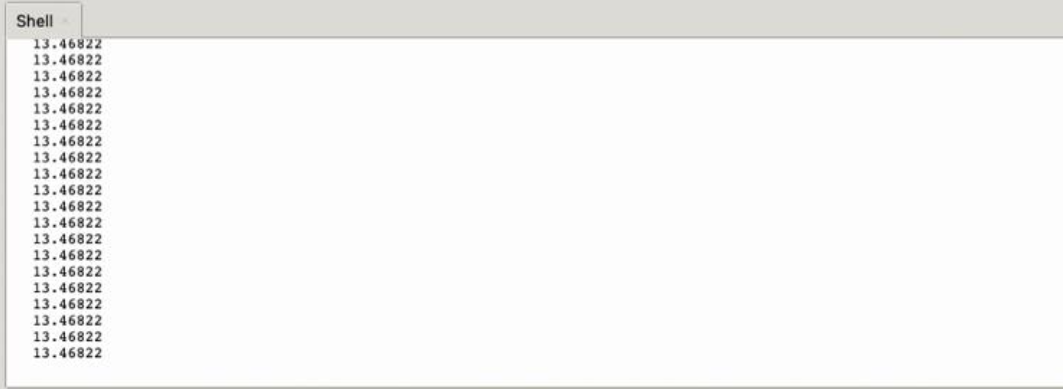
\includegraphics[width=1\linewidth]{img/1.png}
    \caption{}
\end{figure}
\newpage
%%%%%%%%%%%%%%%%%%%%%%%%%%%%%%%%%%%%%%%%%%%
\subsection{Ejercicio 2}
Realizar un programa que despliegue en la consola de Thonny el resultado de la conversión y el voltaje generado por el potenciómetro; actualizar cada segundo.

\begin{figure}[ht!]
    \centering
    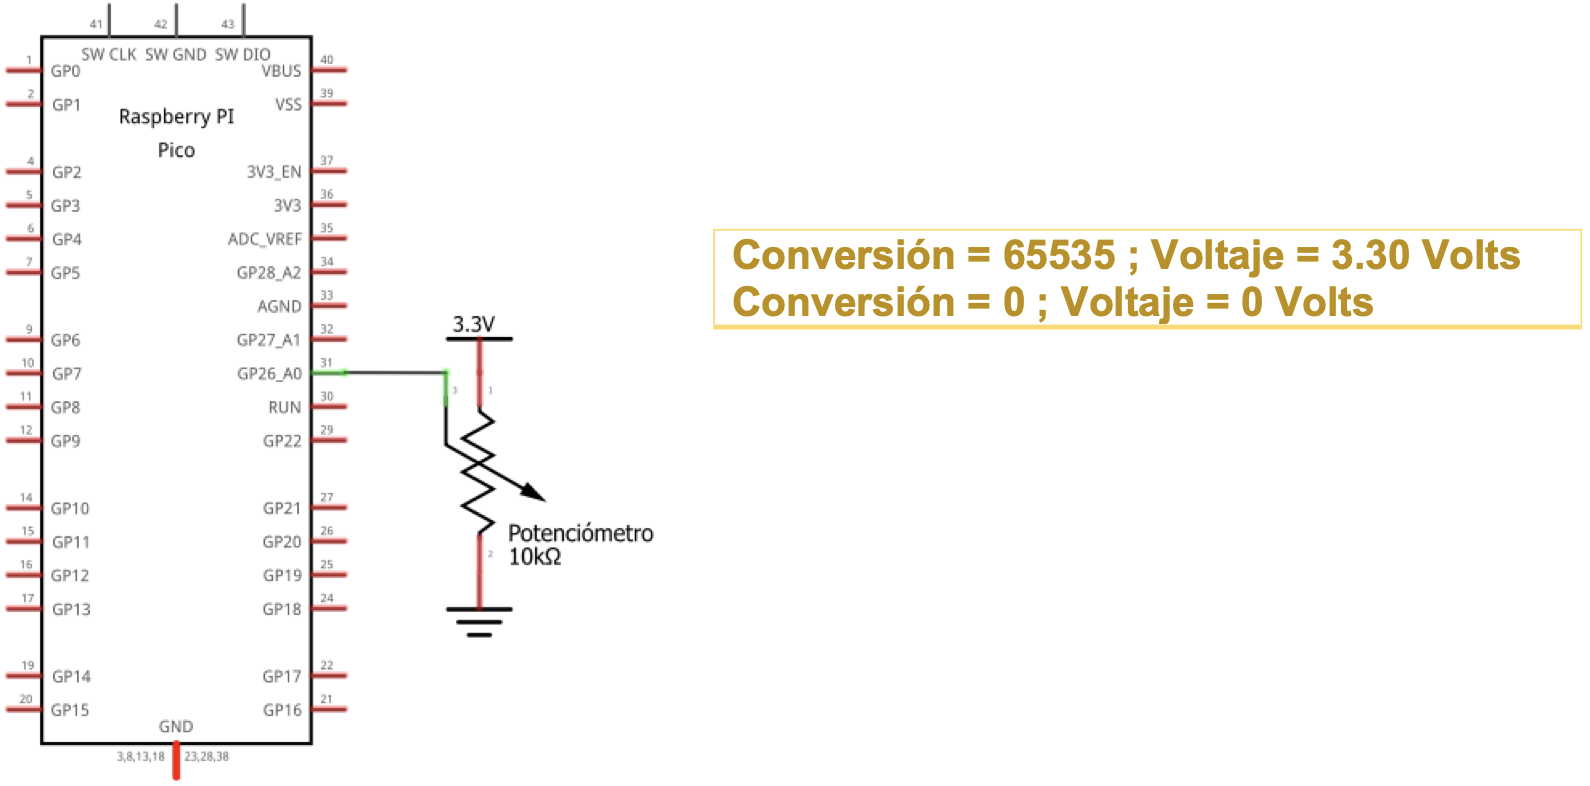
\includegraphics[width=0.9\linewidth]{pics/2.png}
    \caption{Circuito y ejecución; actividad 2}
\end{figure}

\subsubsection{Pseudo Código}

\begin{algorithm}[H]

\SetAlgoLined
\caption{Lectura de potenciómetro}

Inicializar ADC en GPIO26\;
Mientras el programa esté en ejecución hacer\;
\Indp
Leer valor analógico\;
Convertir a voltaje\;
Mostrar valor y voltaje en consola\;
Esperar 1 segundo\;
\Indm

\end{algorithm}

\subsubsection{Desarrollo}
\begin{lstlisting}
from machine import ADC
import time

pot = ADC(26)

while True:
    valor = pot.read_u16()
    voltaje = valor * (3.3 / 65535)

    print("Valor ADC:", valor)
    print("Voltaje:", voltaje)
    print("------------------")
    time.sleep(1)
\end{lstlisting}

\subsubsection{Análisis de resultados}
El programa permite leer el valor analógico generado por el potenciómetro mediante el ADC del microcontrolador.
Se convierte la señal a voltaje y se muestra en la consola cada segundo.
Al girar el potenciómetro se observa el cambio del voltaje, lo que confirma el correcto funcionamiento del divisor de voltaje.

\begin{figure}[ht!]
    \centering
    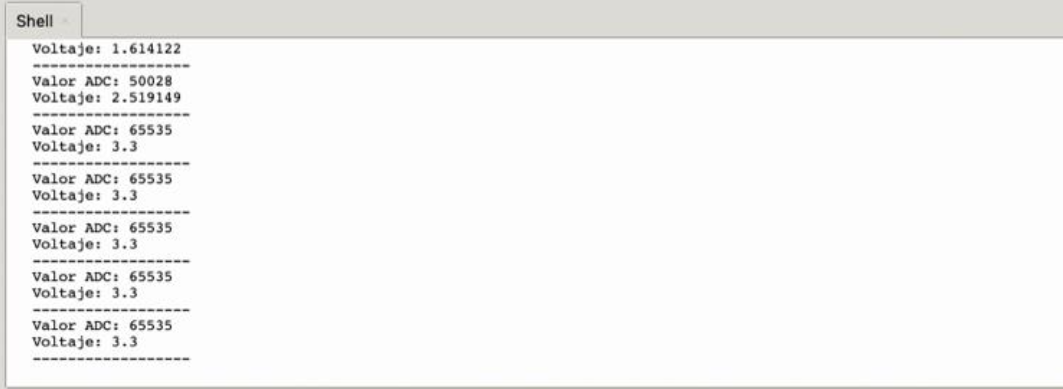
\includegraphics[width=1\linewidth]{img/2.png}
    \caption{}
\end{figure}
\newpage
%%%%%%%%%%%%%%%%%%%%%%%%%%%%%%%%%%%%%%%%%%%
\subsection{Ejercicio 3}
Empleando el divisor de voltaje generado por la foto-resistencia; tomar la lectura de voltaje, registrar el máximo y mínimo obtenido, fijar un valor de referencia. Mientras la lectura es menor a la referencia, mantenga en bajo el GPIO7 y cuando sobrepase el valor configurado lo ponga en alto.

\begin{figure}[ht!]
    \centering
    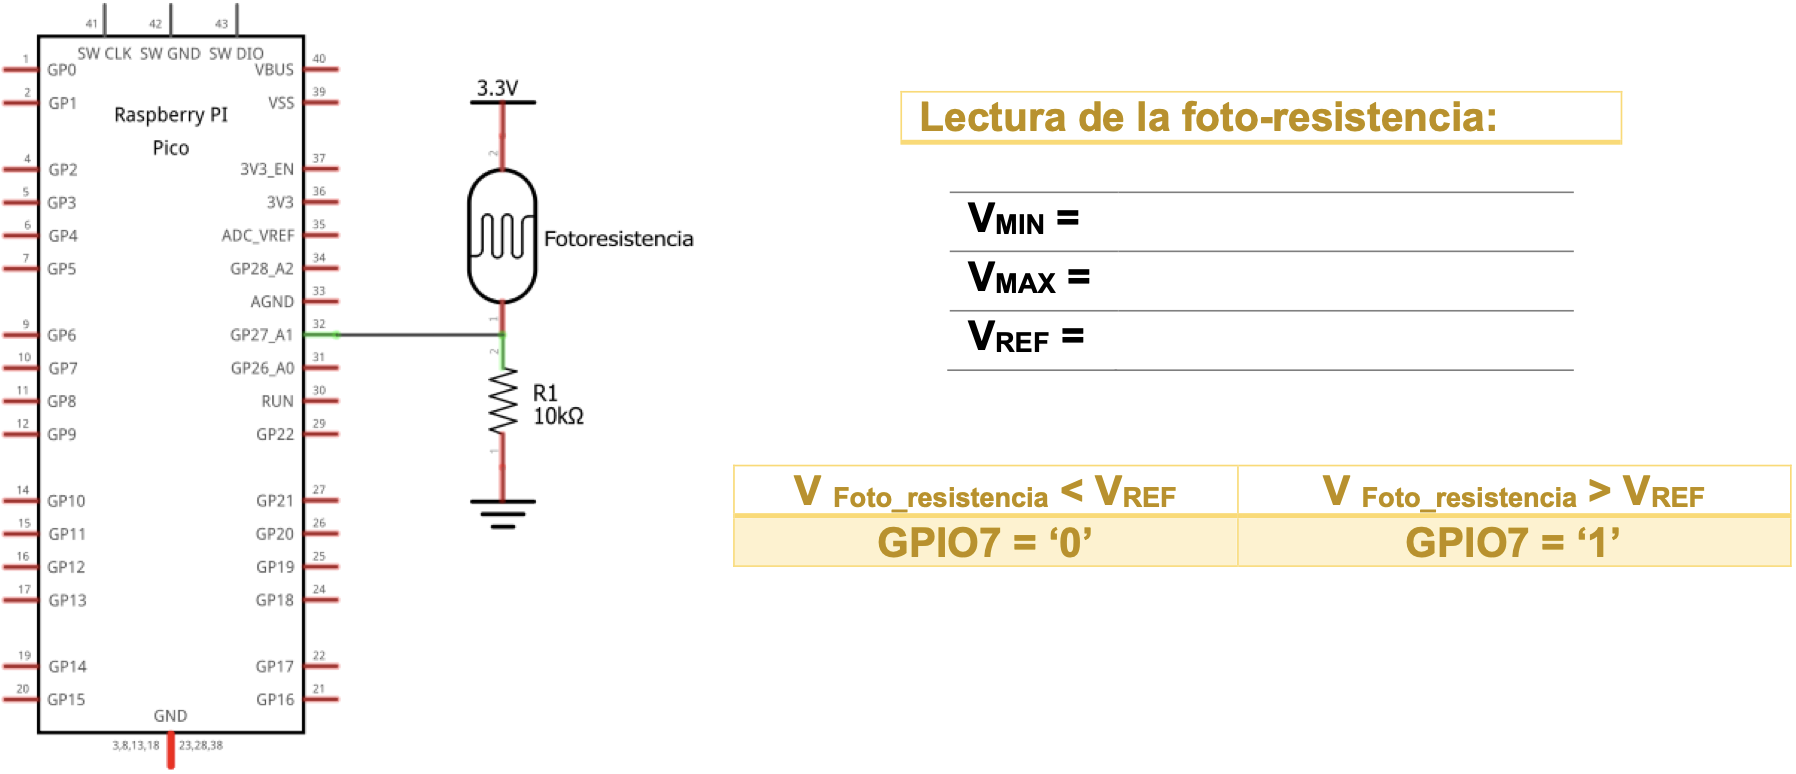
\includegraphics[width=\linewidth]{pics/3.png}
    \caption{Circuito y ejecución; actividad 2}
\end{figure}

\subsubsection{Pseudo Código}

\begin{algorithm}[H]

\SetAlgoLined
\caption{Control GPIO con fotoresistencia}

Inicializar ADC en GPIO26\;
Inicializar GPIO7 como salida\;
Definir valor de referencia\;

Mientras el programa esté en ejecución hacer\;
\Indp
Leer voltaje de la fotoresistencia\;
Si el voltaje es menor a la referencia\;
\Indp
GPIO7 = 0\;
\Indm
Si no\;
\Indp
GPIO7 = 1\;
\Indm
\Indm

\end{algorithm}
\subsubsection{Desarrollo}

\begin{lstlisting}
from machine import ADC, Pin
import time

ldr = ADC(26)
gpio7 = Pin(7, Pin.OUT)

referencia = 1.5

while True:

    valor = ldr.read_u16()
    voltaje = valor * (3.3 / 65535)

    if voltaje < referencia:
        gpio7.value(0)
    else:
        gpio7.value(1)

    print(voltaje)

    time.sleep(1)
\end{lstlisting}

\subsubsection{Análisis de resultados}
El sistema utiliza una fotoresistencia para detectar cambios de luz.
Cuando la iluminación es baja, el voltaje disminuye y el GPIO7 se mantiene en bajo.
Cuando la luz aumenta y supera el valor de referencia, el GPIO7 se activa.
Esto permite implementar un sistema de detección de luz o encendido automático.


\begin{figure}[ht!]
    \begin{minipage}{0.3\textwidth}
        \centering
        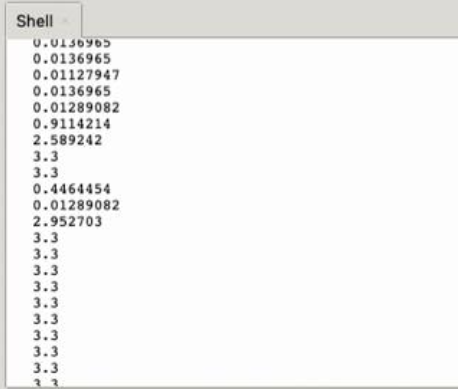
\includegraphics[width=\linewidth]{img/3a.png}
        \caption{}        
    \end{minipage}
    \hfill
    \begin{minipage}{0.6\textwidth}
    \centering
    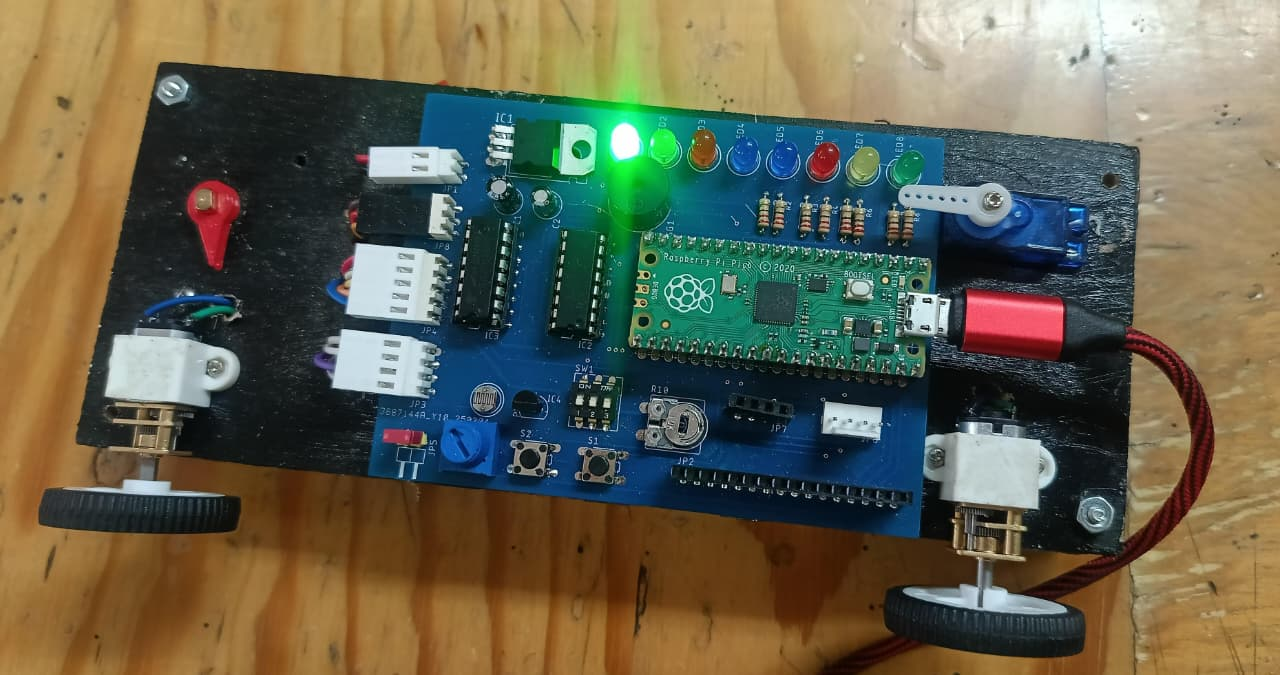
\includegraphics[width=\linewidth]{img/3b.png}
    \caption{}
    \end{minipage}
\end{figure}

\newpage

%%%%%%%%%%%%%%%%%%%%%%%%%%%%%%%%%%%%%%%%%%%
\subsection{Ejercicio 4}
Realizar un programa que muestre el valor de temperatura tanto en oC como oF, en la  consola de Thonny del sensor interno y del sensor TMP36; indicando cual de ellos tiene valor mayor al otro. 
\begin{figure}[ht!]
    \centering
    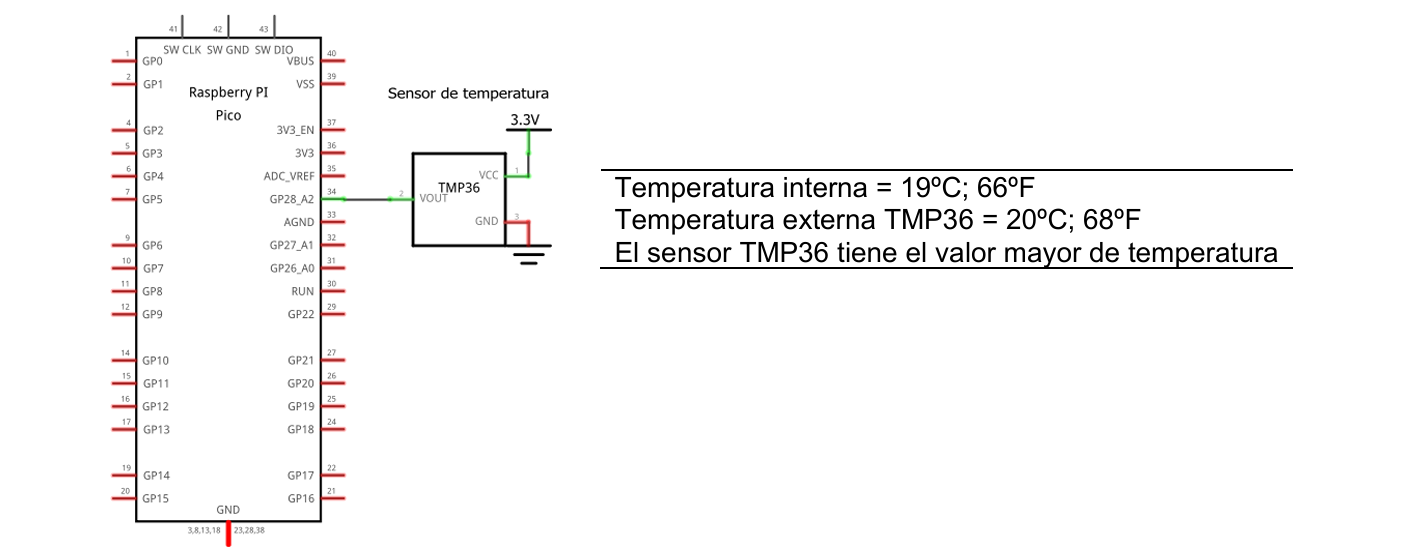
\includegraphics[width=1\linewidth]{pics/4.png}
\end{figure}

\subsubsection{Pseudo Código}

\begin{algorithm}[H]

\SetAlgoLined
\caption{Comparación de sensores de temperatura}

Inicializar ADC4 sensor interno\;
Inicializar ADC26 TMP36\;

Mientras el programa esté en ejecución hacer\;
\Indp
Leer temperatura interna\;
Leer temperatura TMP36\;
Convertir a Celsius\;
Convertir a Fahrenheit\;

Comparar temperaturas\;

Mostrar resultados\;

\Indm

\end{algorithm}

\subsubsection{Desarrollo}
\begin{lstlisting}
from machine import ADC
import time

sensor_int = ADC(4)
tmp36 = ADC(26)

while True:

    # Sensor interno
    v1 = sensor_int.read_u16() * (3.3 / 65535)
    t1 = 27 - (v1 - 0.706) / 0.001721

    # TMP36
    v2 = tmp36.read_u16() * (3.3 / 65535)
    t2 = (v2 - 0.5) * 100

    f1 = (t1 * 9/5) + 32
    f2 = (t2 * 9/5) + 32

    print("Sensor interno:", t1, "C", f1, "F")
    print("TMP36:", t2, "C", f2, "F")

    if t1 > t2:
        print("Sensor interno mayor")
    else:
        print("TMP36 mayor")

    print("----------------")

    time.sleep(1)
\end{lstlisting}
\subsubsection{Análisis de resultados}
El programa mide la temperatura usando dos sensores distintos.
Se convierten los valores a grados Celsius y Fahrenheit y se comparan los resultados.
Generalmente el TMP36 ofrece una medición más estable que el sensor interno, ya que el sensor interno puede variar por el calentamiento del microcontrolador.

\begin{figure}[ht!]
    \centering
    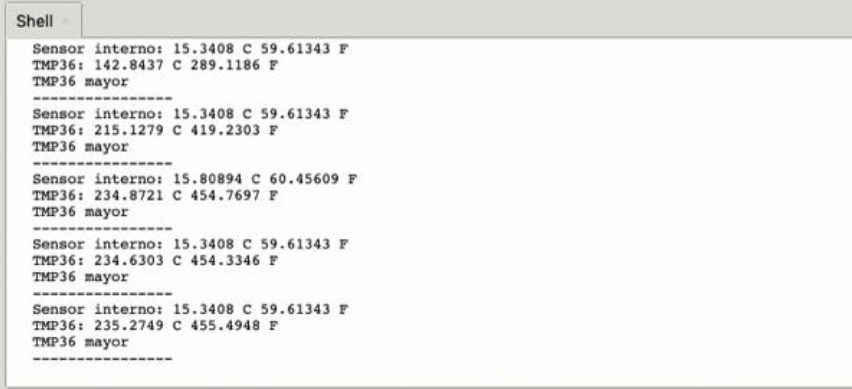
\includegraphics[width=1\linewidth]{img/4.png}
    \caption{}
\end{figure}
\newpage
%%%%%%%%%%%%%%%%%%%%%%%%%%%%%%%%%%%%%%%%%%%
\subsection{Ejercicio 5}
Escribir el siguiente programa, comentar e indicar que hace: 
\begin{lstlisting}
from machine import Pin, PWM
import time
pwm=PWM(Pin(1))
pwm.freq(1000)

while True:
    for duty in range(0, 65535, 500):
        pwm.duty_u16(duty)
        time.sleep(0.05)
    pwm.duty_u16(0)
    time.sleep(2)
\end{lstlisting}
\subsubsection{Pseudo Código}

\begin{algorithm}[H]

\SetAlgoLined
\caption{Generación de PWM}

Inicializar PWM en GPIO1\;
Configurar frecuencia 1000 Hz\;

Mientras el programa esté en ejecución hacer\;
\Indp
Incrementar duty cycle\;
Aplicar PWM\;
Esperar\;

Apagar PWM\;
Esperar 2 segundos\;

\Indm

\end{algorithm}

\subsubsection{Desarrollo}

\begin{lstlisting}
from machine import Pin, PWM
import time

pwm = PWM(Pin(1))
pwm.freq(1000)

while True:

    for duty in range(0, 65535, 500):
        pwm.duty_u16(duty)
        time.sleep(0.05)

    pwm.duty_u16(0)
    time.sleep(2)
\end{lstlisting}
\newpage

\subsubsection{Análisis de resultados}
El programa genera una señal PWM que incrementa gradualmente su ciclo de trabajo.
Esto permite controlar la intensidad de un LED o la velocidad de un motor.
Después de alcanzar el máximo, el PWM se apaga y espera dos segundos antes de reiniciar el ciclo.

\begin{figure}[ht!]
    \centering
    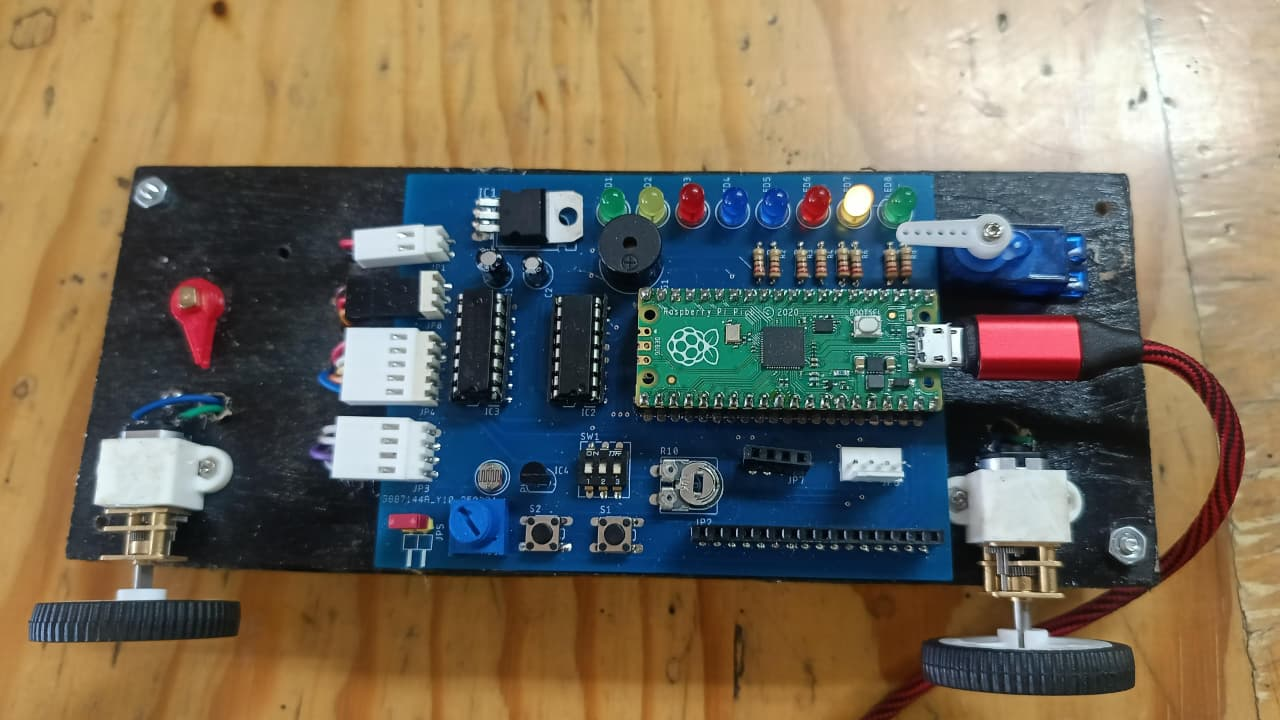
\includegraphics[width=1\linewidth]{img/5.png}
    \caption{}
\end{figure}
\newpage
%%%%%%%%%%%%%%%%%%%%%%%%%%%%%%%%%%%%%%%%%%%
\subsection{Ejercicio 6}
Modificar el programa para que incremente y decremente de manera automática el valor 
de PWM en la terminal GPIO0 y refleje el valor inverso en el pin GPIO1.

\begin{figure}[ht!]
    \centering
    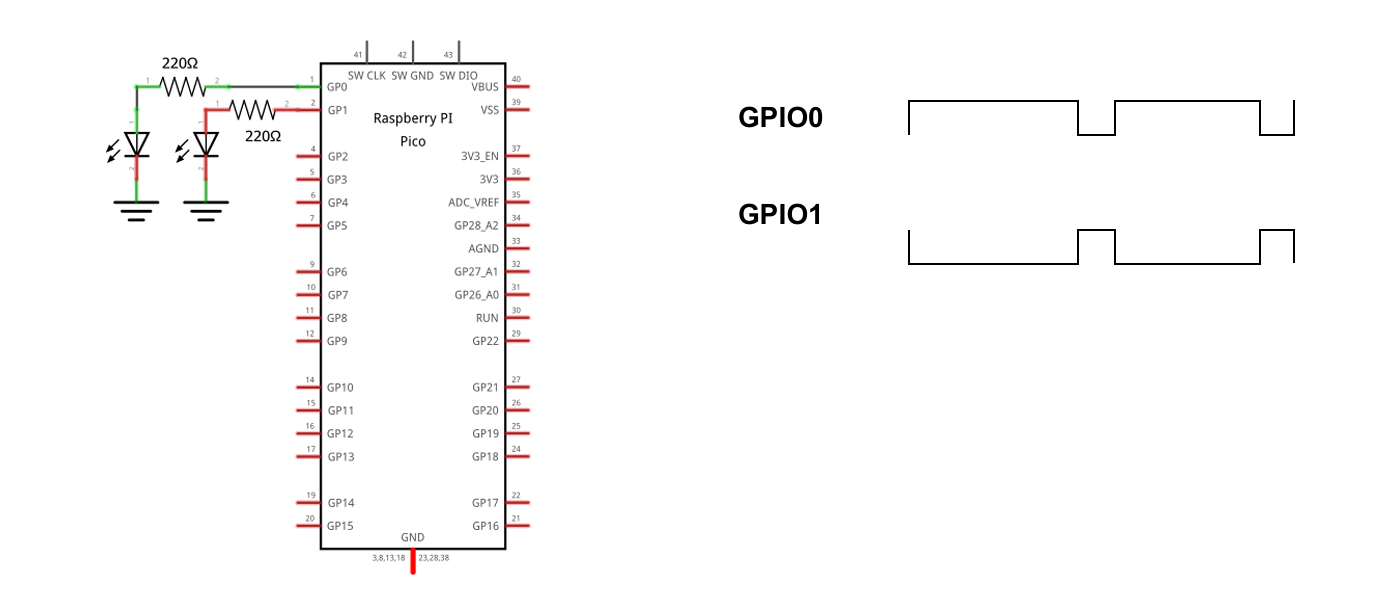
\includegraphics[width=1\linewidth]{pics/6.png}
    \caption{Circuito y oscilograma requerido; actividad 6}
\end{figure}
\subsubsection{Pseudo Código}

\begin{algorithm}[H]

\SetAlgoLined
\caption{PWM inverso en GPIO0 y GPIO1}

Inicializar GPIO0 como PWM\;
Inicializar GPIO1 como PWM\;

Configurar frecuencia de 1000 Hz en ambos pines\;

Mientras el programa esté en ejecución hacer\;
\Indp

Para duty desde 0 hasta 65535 hacer\;
\Indp
PWM GPIO0 = duty\;
PWM GPIO1 = 65535 - duty\;
Esperar 0.05 segundos\;
\Indm

Para duty desde 65535 hasta 0 hacer\;
\Indp
PWM GPIO0 = duty\;
PWM GPIO1 = 65535 - duty\;
Esperar 0.05 segundos\;
\Indm

\Indm

\end{algorithm}
\subsubsection{Desarrollo}

\begin{lstlisting}
from machine import Pin, PWM
import time

pwm0 = PWM(Pin(0))
pwm1 = PWM(Pin(1))

pwm0.freq(1000)
pwm1.freq(1000)

while True:

    for duty in range(0, 65535, 500):

        pwm0.duty_u16(duty)
        pwm1.duty_u16(65535 - duty)

        time.sleep(0.05)

    for duty in range(65535, 0, -500):

        pwm0.duty_u16(duty)
        pwm1.duty_u16(65535 - duty)

        time.sleep(0.05)
\end{lstlisting}

\subsubsection{Análisis de resultados}
El PWM de GPIO0 incrementa mientras el GPIO1 decrece.
Esto genera señales inversas, como se observa en los leds.
\begin{figure}[ht!]
    \centering
    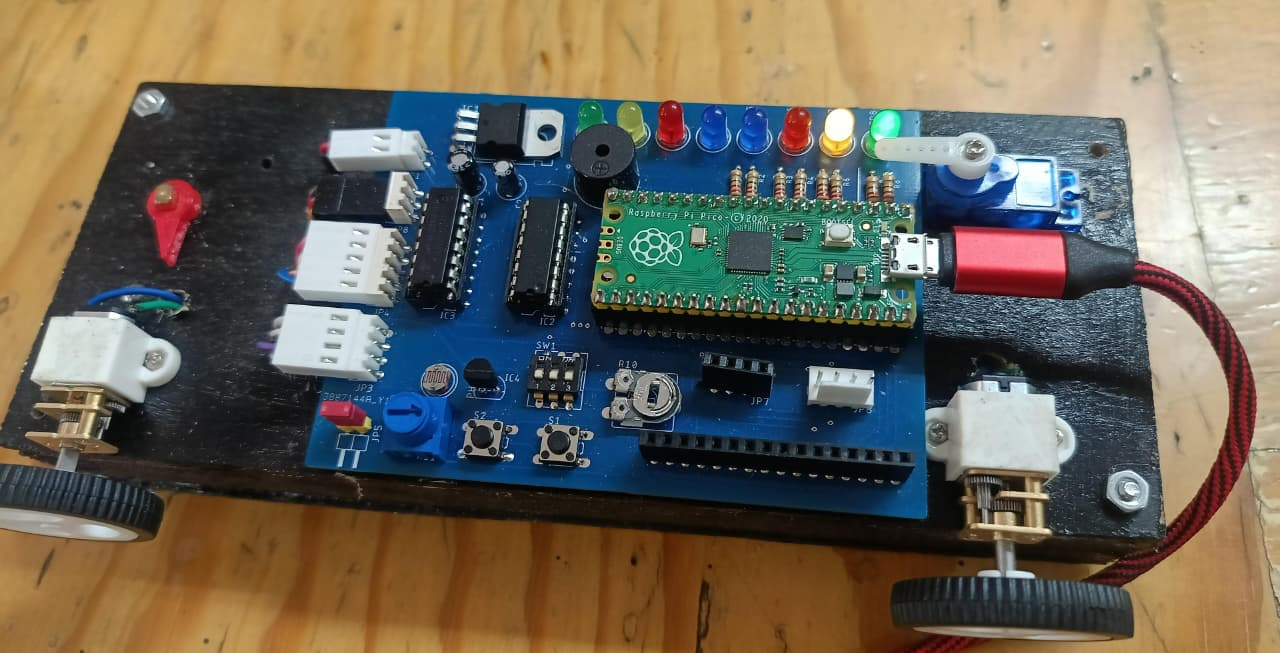
\includegraphics[width=1\linewidth]{img/6.png}
    \caption{}
\end{figure}
\newpage
%%%%%%%%%%%%%%%%%%%%%%%%%%%%%%%%%%%%%%%%%%%
\subsection{Ejercicio 7}
Realizar las modificaciones necesarias para realizar el control anterior pero ahora a través de la selal analógica proveniente del potenciómetro. 
\begin{figure}[ht!]
    \centering
    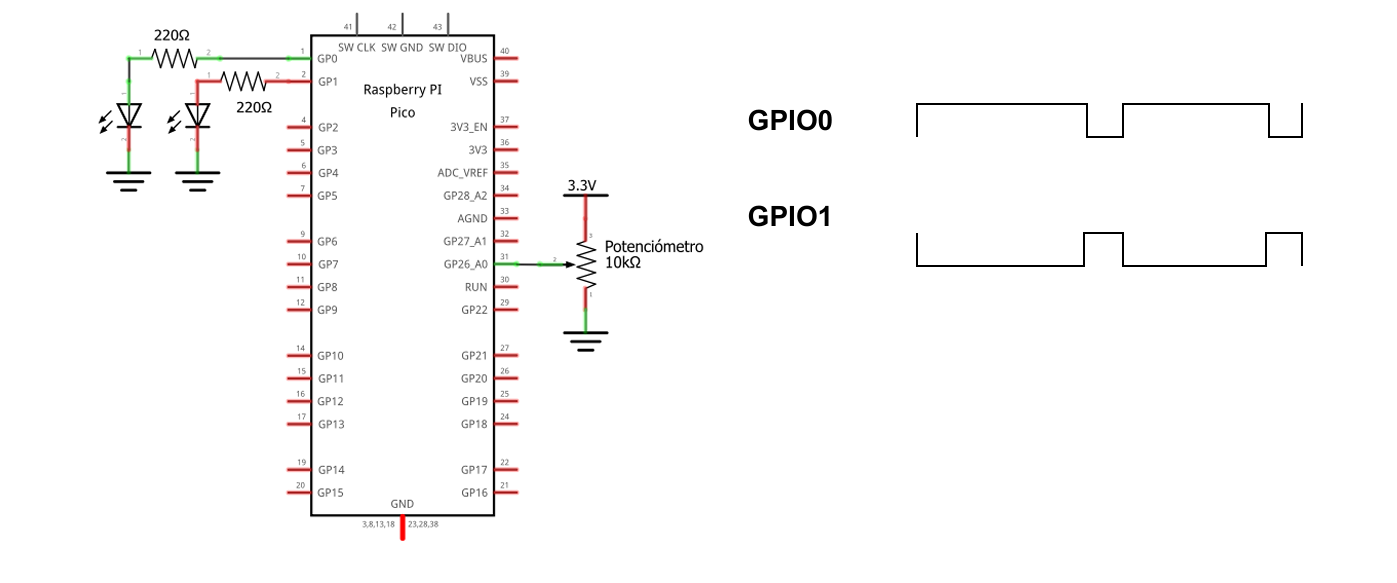
\includegraphics[width=1\linewidth]{pics/7.png}
    \caption{Control PWM por medio de entrada analógica; actividad 7}
\end{figure}
\subsubsection{Pseudo Código}

\begin{algorithm}[H]

\SetAlgoLined
\caption{Control PWM con potenciómetro}

Inicializar ADC en GPIO26 (potenciómetro)\;

Inicializar GPIO0 como PWM\;
Inicializar GPIO1 como PWM\;

Configurar frecuencia de 1000 Hz en ambos pines\;

Mientras el programa esté en ejecución hacer\;
\Indp

Leer valor del potenciómetro\;

PWM GPIO0 = valor leído\;

PWM GPIO1 = 65535 - valor leído\;

Esperar 0.1 segundos\;

\Indm

\end{algorithm}

\subsubsection{Desarrollo}

\begin{lstlisting}
from machine import ADC, Pin, PWM
import time

pot = ADC(26)

pwm0 = PWM(Pin(0))
pwm1 = PWM(Pin(1))

pwm0.freq(1000)
pwm1.freq(1000)

while True:

    valor = pot.read_u16()

    pwm0.duty_u16(valor)
    pwm1.duty_u16(65535 - valor)

    time.sleep(0.1)
\end{lstlisting}

\subsubsection{Análisis de resultados}
El potenciómetro controla directamente el PWM.
Al girarlo, un PWM aumenta mientras el otro disminuye, generando una señal inversa controlada manualmente.

\begin{figure}[ht!]
    \centering
    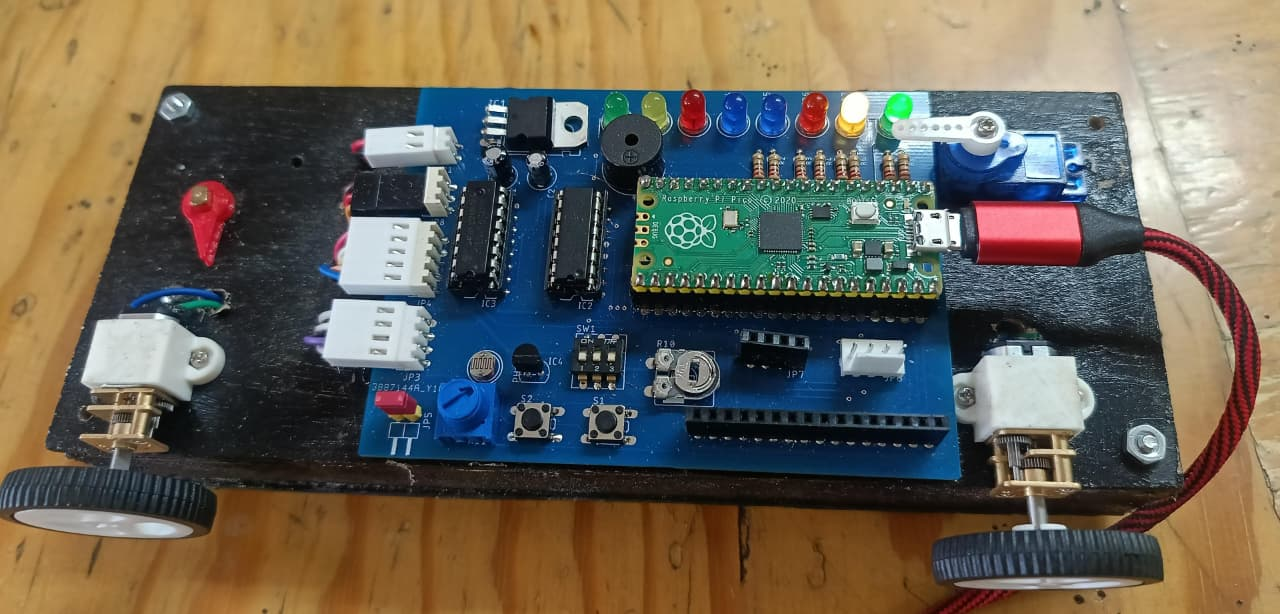
\includegraphics[width=1\linewidth]{img/7.png}
    \caption{}
\end{figure}
%%%%%%%%%%%%%%%%%%%%%%%%%%%%%%%%%%%%%%%%%%%
